\documentclass[10pt]{report}

\usepackage[utf8]{inputenc} % Required for inputting international characters
\usepackage[T1]{fontenc} % Output font encoding for international characters
% \usepackage[demo]{graphicx} % images % get rid of [demo] for black box removal
\usepackage{graphicx} % images % get rid of [demo] for black box removal
\usepackage{fancyhdr} % headers and footers
\usepackage{parskip} % paragraph
\usepackage{geometry} % page size
% \usepackage{hyperref} % Links
% \usepackage{pdflscape} % making a page landscape
\usepackage{xcolor}
\usepackage[shortlabels]{enumitem}
\usepackage{multirow}
\usepackage{listings}
\usepackage{titlesec}
\usepackage{float} % to place figures in place
\usepackage{xurl}

% colors
\usepackage{xcolor}
\definecolor{mygrey}{RGB}{200, 200, 200}


% Helvetica as font
\usepackage[scaled]{helvet}
\renewcommand\familydefault{\sfdefault} 
% \usepackage[scaled=0.8]{FiraMono}

\graphicspath{{../images/}}

\titleformat{\chapter}[display]
  {\normalfont\bfseries}{}{0pt}{\Huge}

% margins and page size
\geometry{
a4paper,
left=30mm,
top=25mm,
right=30mm,
bottom=25mm
}

% \lstset{
%   basicstyle=\ttfamily,
%   columns=fullflexible,
%   frame=single,
%   breaklines=true,
%   postbreak=\mbox{\textcolor{red}{$\hookrightarrow$}\space},
% }

\definecolor{mygreen}{rgb}{0,0.6,0}
\definecolor{mygray}{rgb}{0.5,0.5,0.5}
\definecolor{mymauve}{rgb}{0.58,0,0.82}
% code formatting
\lstset{ %
  backgroundcolor=\color{white},   % choose the background color
  basicstyle=\ttfamily\footnotesize,    % fixed spaced font familyy  &  size of fonts used for the code
  breaklines=true,                 % automatic line breaking only at whitespace
  postbreak=\mbox{\textcolor{red}{$\hookrightarrow$}\space},
  captionpos=b,                    % sets the caption-position to bottom
  commentstyle=\color{mygreen},    % comment style
  escapeinside={\%*}{*)},          % if you want to add LaTeX within your code
  keywordstyle=\color{blue},       % keyword style
  stringstyle=\color{mymauve},     % string literal style
  frame=single,                    % border
}


\pagestyle{fancy}
\fancyhf{}
\rhead{Aum Patel}
\cfoot{\thepage}

% % in line code with bg command
% \newcommand{\code}[1][]{%
% \colorbox{mygrey}{\lstinline{#1}}%
% }

\begin{document}

%title
\author{Aum Patel - 180000492}
\title{Computer Graphics}
\maketitle

\section*{Overview}
The project I have created is based around a 'candy cane' style theme, where everything is vibrant and multi-coloured. 

\section*{Annotated Game Scene}

\begin{figure}[H]
    \begin{minipage}{.5\textwidth}
        \centering
        \fbox{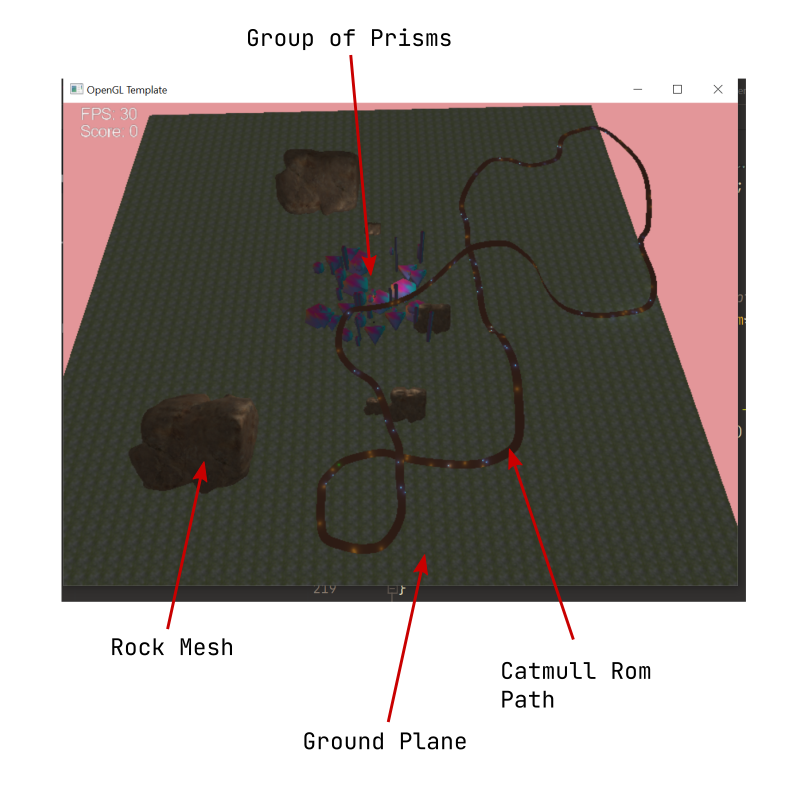
\includegraphics[width = 7cm ]{Zoomed Out Labelling.png}}
        \caption{Top Down view of the game scene, zoomed out}
    \end{minipage}
    \begin{minipage}{.5\textwidth}
        \centering
        \fbox{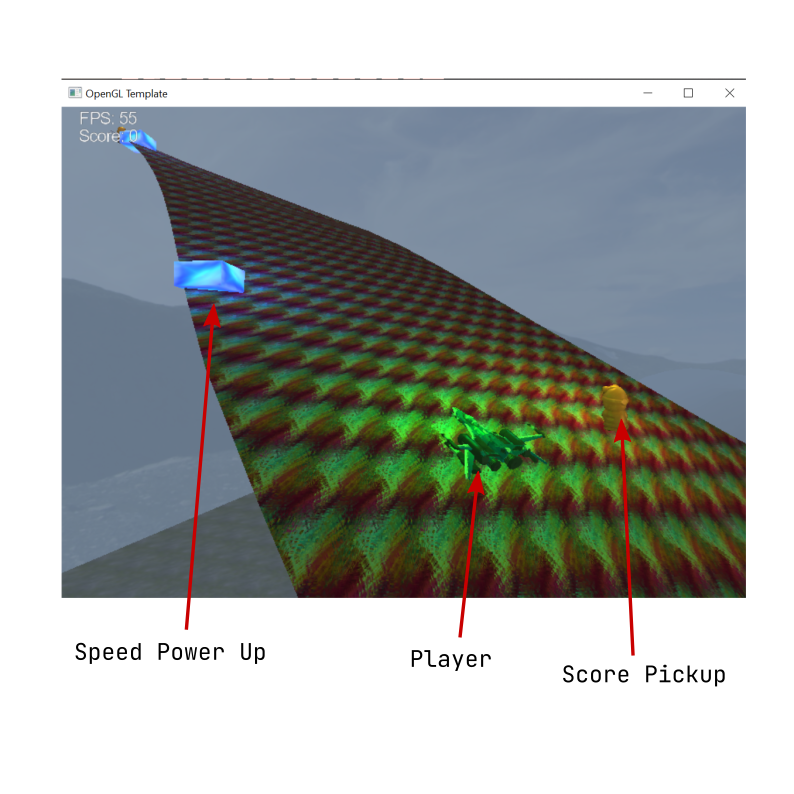
\includegraphics[width = 7cm ]{Player_Pickups_Zoomed_In.png}}
        \caption{Close view of the player, speed power up and score power up}
    \end{minipage}
\end{figure}

\section*{User Guide}
    The goal of the game is to collect as many chocolate santa clause's as possible to get a high score. The player can pick up the blue pointed shape to gain a temporary speed boost.
    \begin{table}[H]
        \begin{center}
            \begin{tabular}{|l|l|}
            \hline
            \textbf{Controls}    & \textbf{Description}  \\
            \hline
              &  \\[0.5pt]
              Up Arrow    & Accelerate                   \\[10pt]
              Down Arrow  & Deccelerate                  \\[10pt]
              Left Arrow  & Move Left                    \\[10pt]
              Right Arrow & Move Right                   \\[10pt] 
              F           & Switch Camera View           \\[10pt]
              W A S D     & Camera Movement in Free Roam \\[10pt]
            \hline
            \end{tabular}
            \caption{Controls for the game}
        \end{center}
    \end{table}


\section*{Route and Camera}

% Route
\subsection*{Route}
% Planning
To plan out the path, Blender was used, as this provided an easier time visualising it over pen and paper. After sketching, I measured and listed the vertices out which are then used in the Catmull Rom \colorbox{mygrey}{\lstinline{SetControlPoints()}} method; the measurement displayed in the image below are rounded to the nearest fifth, as the Blender measure tool does not snap. 
\begin{figure}[H]
    \centering
    \fbox{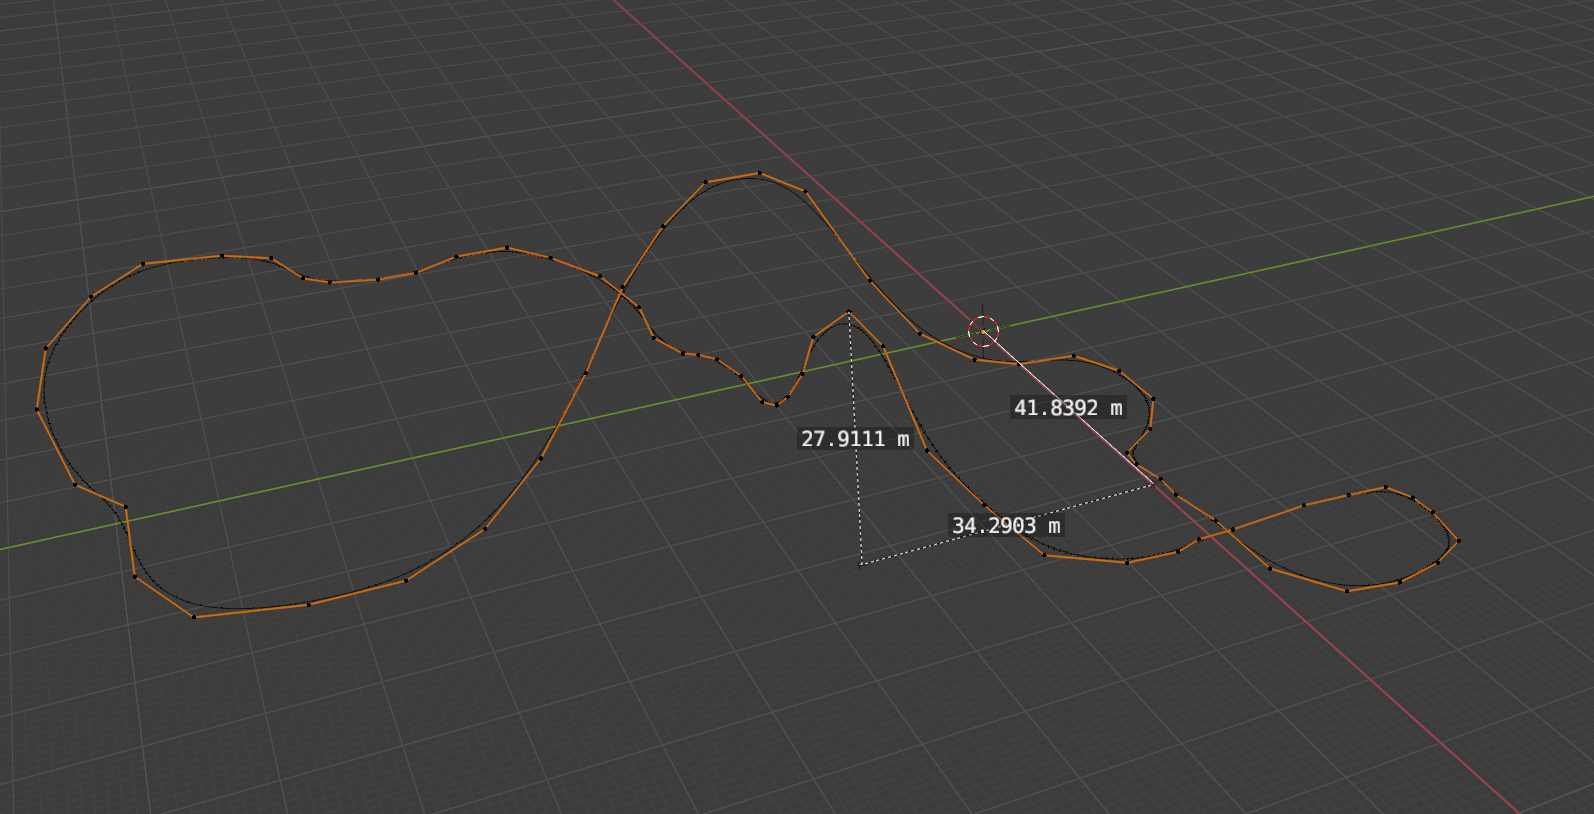
\includegraphics[width = 14cm]{Path_Plan_in_Blender.png}}
    \caption{Path Sketched out in Blender}
\end{figure}

% Adding Control Points
When adding the points into the \colorbox{mygrey}{\lstinline{SetControlPoints()}} method, I decided to create some parameters and add/multiply those to the vertices I was adding in, these parameters were a scalar value on the xyz axis and an offset value on the xyz (which is multiplied by the scalar before being applied to the control points). This way I could move the path around freely without needing to adjust the vertices.


% \begin{lstlisting}[language=c]
% SetControlPoints(){
%     // parameters to adjust the scaling and positioning of the path.
%     const float xScale = 10.f;
%     const float zScale = 10.f;
%     const float yScale = 10.f;
%     const float xOffset = 0 * xScale;
%     const float zOffset = 0 * zScale;
%     const float yOffset = 10 * yScale;

%     // example for one control point. Total of 70 points
%     m_controlPoints.emplace_back(xOffset + xScale * 59.0, yOffset + yScale * 5.0, zOffset + zScale * 7.0);
% }
% \end{lstlisting}

\subsection*{Camera}
I have implemented 5 camera modes: \textbf{First Person}, \textbf{Third Person}, \textbf{Left Side View}, \textbf{Right Side View} and \textbf{Top View}.

% Switching Camera modes
I switch between them by storing the current \colorbox{mygrey}{\lstinline{cameraType}} as an integer, and have a set of camera modes:
\begin{lstlisting}[language=c]
    static const glm::uint FIRST_PERSON = 0;
    static const glm::uint THIRD_PERSON = 1;
    ... // and so on
\end{lstlisting}
When switching camera mode, I change the camera type and check against this set of constant integers when setting the view of the camera by the spline and place the camera relative to the path with different distance values.

% First Person Camera Mode
I generate a TNB frame in every instance and offset the camera's position relative to the TNB frame to move it along local coordinates. For the \textbf{first person view} I moved it up one value on the bi-normal to place it just above the nose of the spaceship.

For the \textbf{3rd person view}, I moved it even higher, and placed it slightly behind the car so the whole track can be seen. When in 3rd person the camera does not follow the left and right movement of the car like it does in First Person.

For the \textbf{side views} I multiply an positive/negative (for both left/right sides) offset value by the normal and place the camera's 'look at' at the car's position.

Similar with the \textbf{top view}, moving it up on the binormal and having the camera look down at the car.

As well as these views, I still have the free view available to toggle to making it easy to debug.

\section*{HUD, Gameplay and Advanced Rendering}
\subsection*{HUD}
To create the HUD, I chose to use full-screen PNG's that act as sprites in the game and are rendered on top of the rendered frame using a full-screen quad. I created a \colorbox{mygrey}{\lstinline{HudItem}} class which holds one or multiple textures and can be 'bound' to the renderer by passing in an index to the texture wanting rendered; these textures are stored inside a vector. The \colorbox{mygrey}{\lstinline{HudManager}} will then render the many HudItems that are created.

% \begin{lstlisting}[language=c]
% void HudManager::Create() {
%     ...
%     // create a full screen quad
%     ...
%     santa.AddTexture("resources\\textures\\hud\\santa_png\\santa.png");

%     for (int i = 1; i <= 6; ++i) {
%         speedometer.AddTexture("resources\\textures\\hud\\speedometer_png\\speed_" + to_string(i) + ".png");
%     }
%     speedometer.AddTexture("resources\\textures\\hud\\speedometer_png\\speed_boost.png");
% }

% void HudManager::Render(CShaderProgram* shader) {
%     // Draw santa
%     glBindVertexArray(quadVAO);
%     santa.Bind(0);
%     glDrawArrays(GL_TRIANGLES, 0, 6);

%     // Draw Speedometer
%     glBindVertexArray(quadVAO);
%     // will draw the appropriate speedometer texture
%     speedometer.Bind(speedometerIndex);
%     glDrawArrays(GL_TRIANGLES, 0, 6);
% }
% \end{lstlisting}

Below are figures that show how the different hud items are displayed.
\begin{figure}[H]
    \begin{minipage}{.5\textwidth}
        \centering
        \fbox{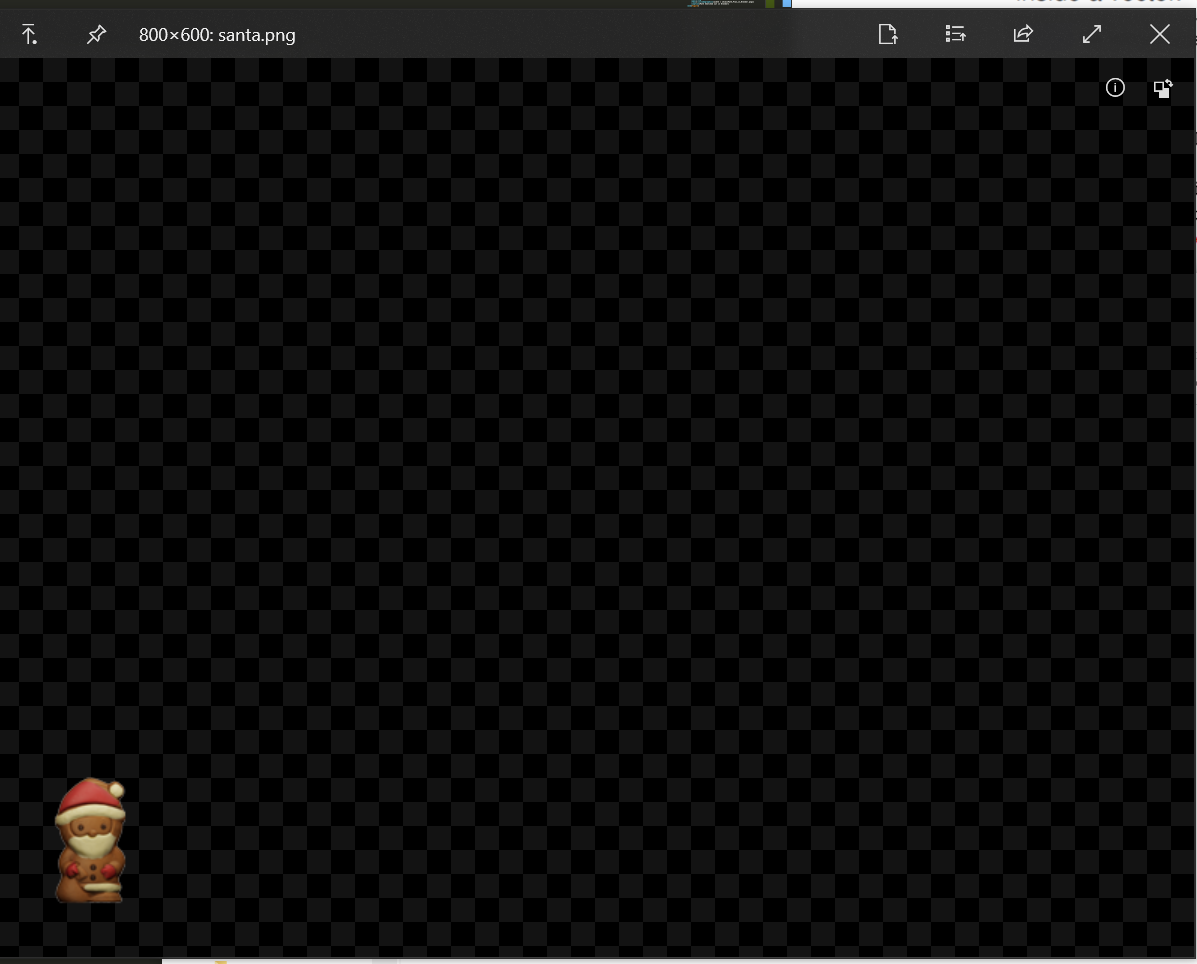
\includegraphics[width = 7cm ]{HUD_Santa.png}}
        \caption{Score HUD Item}
    \end{minipage}
    \begin{minipage}{.5\textwidth}
        \centering
        \fbox{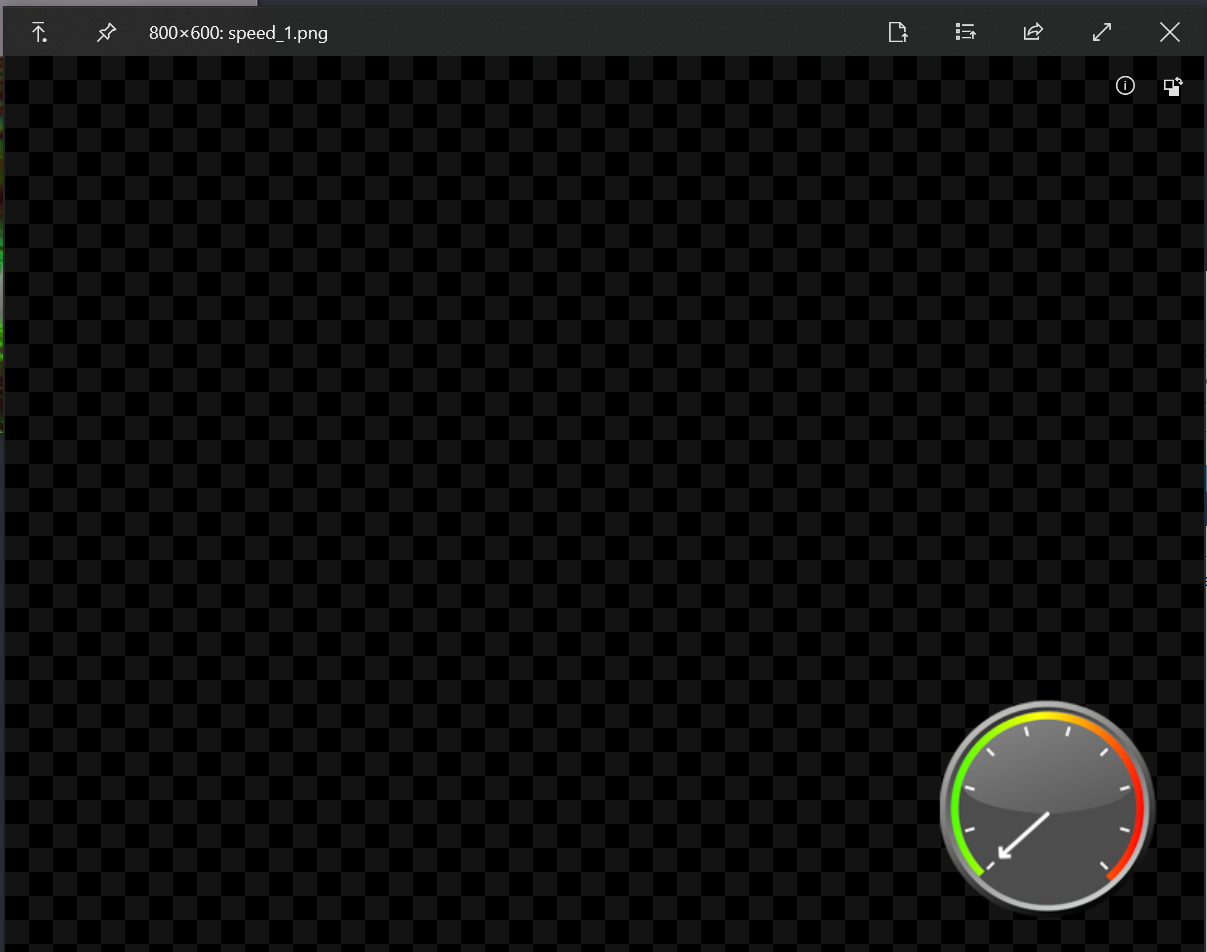
\includegraphics[width = 7cm ]{HUD_Speedometer.png}}
        \caption{Speedometer Hud Item}
    \end{minipage}
\end{figure}

\begin{figure}[H]
    \centering
    \fbox{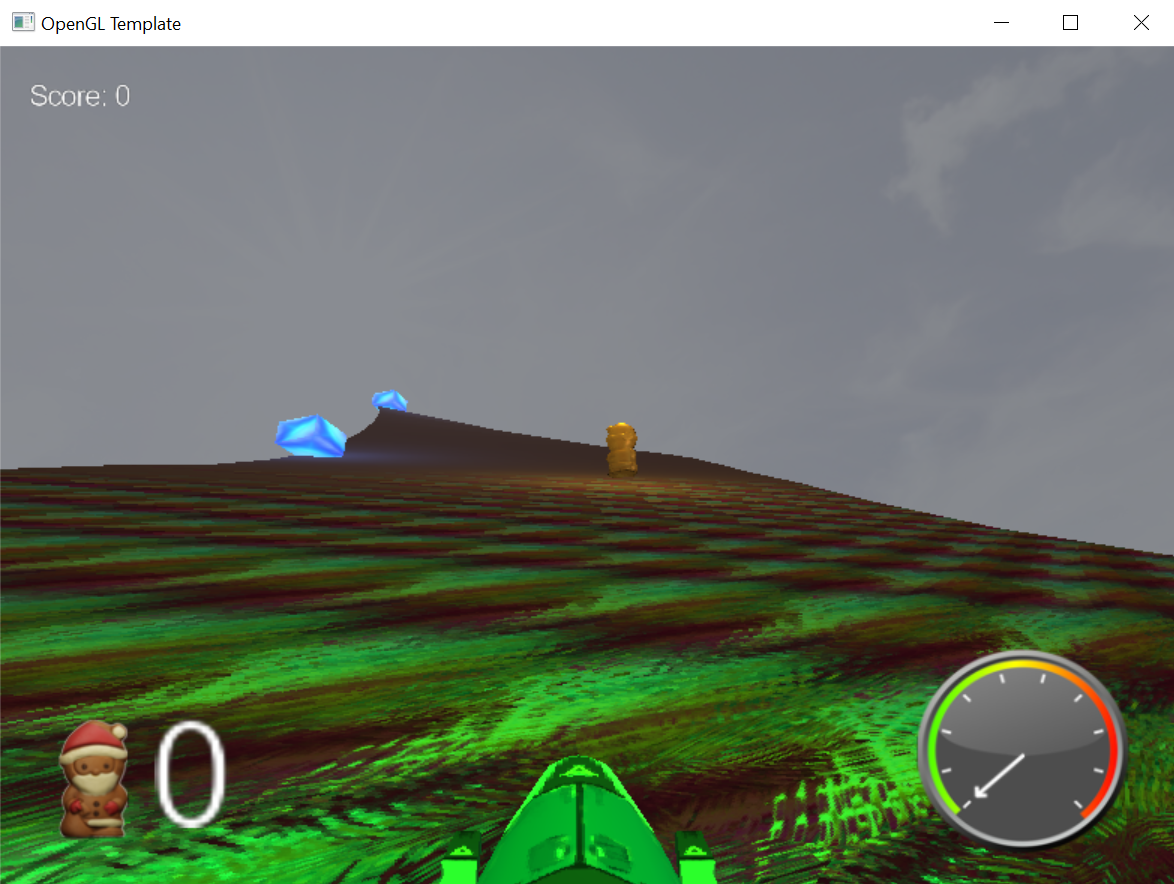
\includegraphics[width = 10cm]{Hud_In_Game.png}}
    \caption{Hud as Displayed in Game}
\end{figure}

As well as the two HUD classes that I created, I also needed a shader to render the 2D elements appropriately. This is a very basic shader that maps the texture's colour to the fragment shader. This is all then rendered after the radial blur in the main Game \colorbox{mygrey}{\lstinline{Render()}} method. This shader was created by taking the radial blur shader, which was already a 2d shader, and removing the values that created the blur effect, essentially giving me a simple 2d shader.

When rendering multiple full-screen elements, the \colorbox{mygrey}{\lstinline{GL_DEPTH_TEST}} had to be disabled, otherwise only the first element rendered will show; disabling depth test is done to avoid 'plane-fighting' where two overlapping faces will clash with each other, however, for the HUD, rendering multiple quads on the same 'plane' needed this to be disabled, to have all elements rendered.

\subsection*{Gameplay}
\subsubsection*{Control}
By pressing the upwards arrow key, the car will accelerate until it reaches the max limit, and vice versa when pressing the down arrow key; when the key is release, the speed will be kept unchanged. This is done by creating a speed value and setting it in both the \textbf{Car} and \textbf{Camera} objects, and changing the value that is being set on the appropriate key presses.

When pressing the Left and Right Arrow keys, the car placed on an offset from the center of the Catmull Rom path. This offset is applied via the TNB frame on the Normal of the car and the camera (only applied to the camera when in First Person View).
\begin{lstlisting}[language=c]
    mPlayerXOffset -= m_dt * mCar->getXOffsetSpeed(); // + for moving right
    mCar->setXOffset(mPlayerXOffset);
    m_pCamera->setXOffset(mCar->getXOffset());
\end{lstlisting}

\subsubsection*{Collision Detection}
The collision detection used in the  game is very simple, however is made easier by using a generalised \colorbox{mygrey}{\lstinline{GameObject}} class, this class contains the collision radius of an object. Any object that is rendered on screen is a child of GameObject. Every frame in the \colorbox{mygrey}{\lstinline{Update()}} loop of my game, I call a function \colorbox{mygrey}{\lstinline{ManageCollisions()}}, which traverses the many vector's that store the positions to render the different game objects and calls \colorbox{mygrey}{\lstinline{CheckCollision(aPos, aRadius, bPos, bRadius)}} that compares the radius between two objects and returns true if they overlap.

When a collision happens, I store the iterator/position inside of the vector of positions and remove it; On doing so, the object in that position will stop rendering, simulating the player picking it up.

\subsubsection*{Gameplay Elements}
Depending on which object it collides with, a different behaviour occurs. For the score pickup, the player's score is incremented by 1, and if it is the speed power up, then \colorbox{mygrey}{\lstinline{mSpeedPowerUpTimer}} is set to 1 seconds, which makes a boost activate. The player just needs to pickup as much chocolate as they can. If they pick up all the points, a game over message will display.
\begin{figure}[H]
    \centering
    \fbox{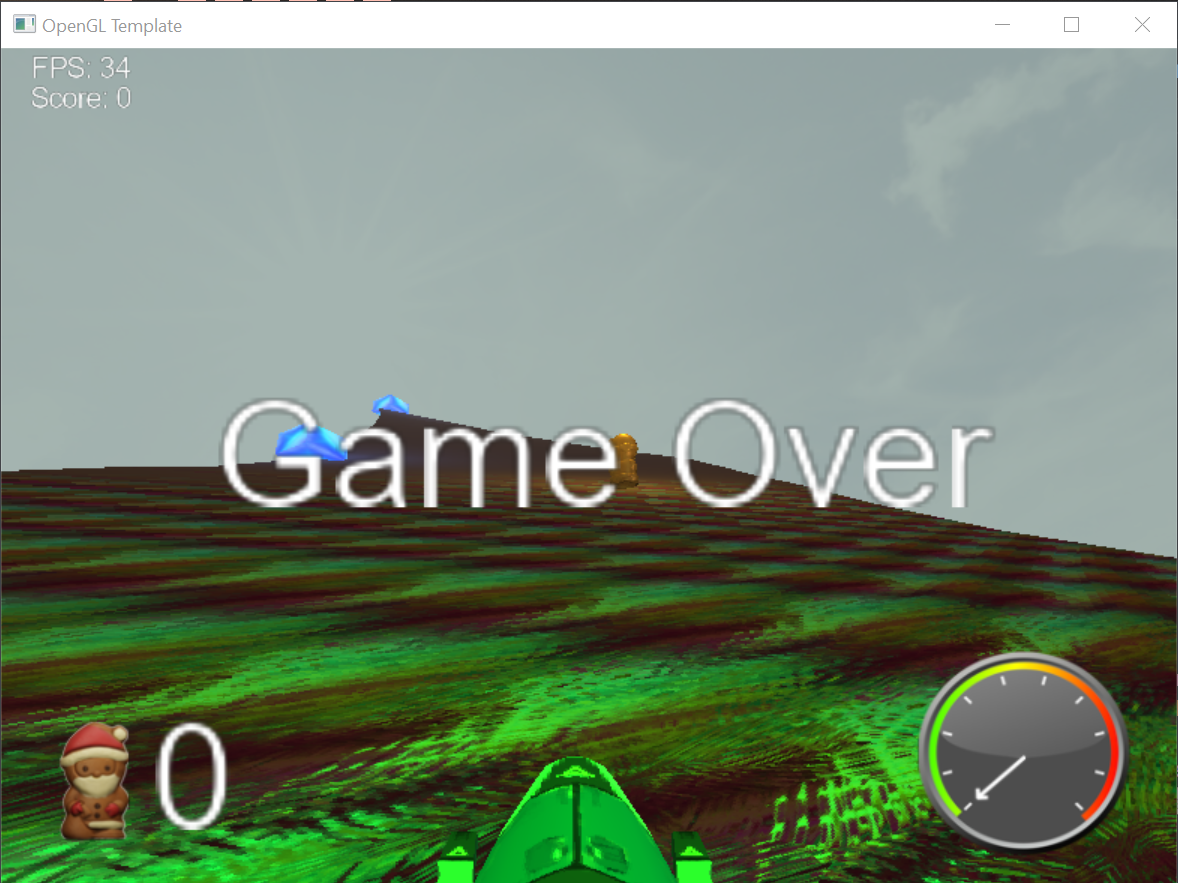
\includegraphics[width = 10cm]{Game_Over_Screen.png}}
    \caption{Game Over Screen}
\end{figure}

\subsection*{Advanced Rendering}

\subsubsection*{Fog}
Two advanced rendering techniques were implemented, the first on was fog. This was achived by following a tutorial \footnote{Tutorial by Thin Matrix for Fog in OpenGL \url{https://youtu.be/qslBNLeSPUc}}. This tutorial described the shader that had to be created, I followed this and adjusted the parameters to get fog that displayed correctly; the \colorbox{mygrey}{\lstinline{mainShader.vert/frag}} was changed to add the fog. As the distance from the player to the object is calculated in the vertex shader per vertex, the distance for large objects, such as the terrain and skybox, is not presented correctly. To rectify this, the density and gradient for both gradient and skybox was lowered to make them visible. 

\begin{figure}[H]
    \centering
    \fbox{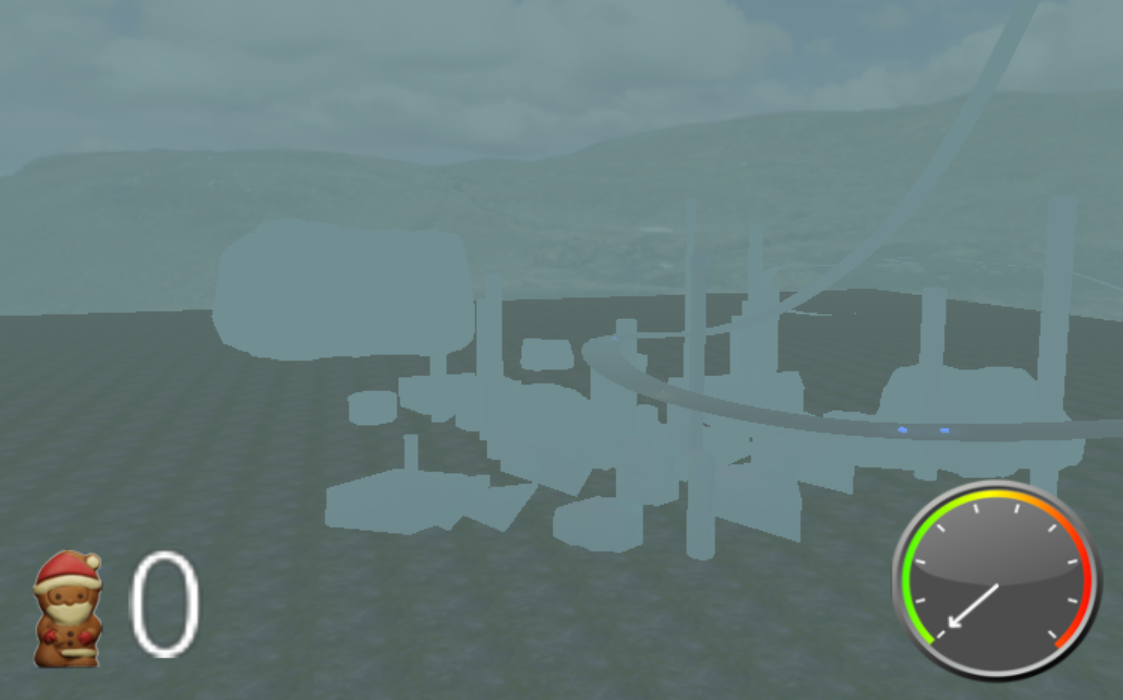
\includegraphics[width = 10cm]{Fog.png}}
    \caption{Fog in game scene}
\end{figure}

To add to the 'candyland' style theme of the game, the colour of the fog was randomly adjusted on the client side, and passed through to fragment shader as the sky colour, giving a nice vibrant ambience.

\subsubsection*{Radial Blur}
The radial blur was achieved by creating a seperate shader files (\colorbox{mygrey}{\lstinline{radialBlur.vert/frag}}) for it. These shaders were created by following the tutorial provided in lecture 7 \footnote{INM376\_2021.L07.pdf, page 55 \url{https://stackoverflow.com/questions/4579020/how-do-i-use-a-glsl-shader-to-apply-a-radial-blur-to-an-entire-scene}}. As this tutorial/post was 10 years old, the shader code had to be ported over to version 400. The fragment shader takes 10 samples 


\end{document}